%\chapter{Fast Convergence in Semi-Anonymous Potential Games}\label{ch2}
%\label{semiAnon chap}

%\noindent\textbf{\emph{When is fast convergence to a near optimal solution possible?}}
\Chapter{Fast Convergence in Semi-Anonymous Potential Games: When is fast convergence to a near optimal solution possible?}\label{ch2}

%Game theoretic learning algorithms have gained traction as a design tool for distributed control systems \cite{Marden2008,Zhu2009,Goto2010,Staudigl2012,Fox2010}.  Here, a static game is repeated over time, and agents revise their strategies based on their objective functions and on observations of other agents' behavior.  Emergent collective behavior for such revision strategies has been studied extensively in the literature, e.g., fictitious play \cite{fp1,fp2,jsfp}, regret matching \cite{Hart2000}, and log-linear learning \cite{Alos-Ferrer2010, Blume1993, Shah2010}.  Although many of these learning rules have desirable asymptotic guarantees, their convergence times either remain uncharacterized or are prohibitively long \cite{Ellison2000, Kandori1993,Shah2010,Hart2010}. Characterizing convergence rates is key to determining whether a distributed algorithm is desirable for system control.

%\todo[inline]{possibly add back in the convergence rates part.}

Emergent collective behavior for game theoretic learning rules has been studied extensively in the literature, e.g., fictitious play \cite{fp1,fp2,jsfp}, regret matching \cite{Hart2000}, and log-linear learning \cite{Alos-Ferrer2010, Blume1993, Shah2010}.  Although many of these learning rules have desirable asymptotic guarantees, their convergence times either remain uncharacterized or are prohibitively long \cite{Ellison2000, Kandori1993,Shah2010,Hart2010}. Characterizing convergence rates is key to determining whether a distributed algorithm is desirable for system control.

In many multi-agent systems, the agent objective functions can be designed to align with the system-level objective function, yielding  a \emph{potential game} \cite{Monderer1996} whose potential function is precisely the system objective function.  Here, the optimal collective behavior of a multi-agent system corresponds to the Nash equilibrium that optimizes the potential function. Hence, learning algorithms which converge to this efficient Nash equilibrium have proven useful for distributed control.

\emph{Log-linear learning} is one algorithm that accomplishes this task \cite{Blume1993}. Log-linear learning is a  {perturbed} best reply process where agents predominantly select the optimal action given their beliefs about other agents' behavior; however, the agents occasionally make mistakes, selecting suboptimal actions with a probability that decays exponentially with respect to the associated payoff loss.  
As noise levels approach zero, the resulting process has a unique stationary distribution with full support on the efficient Nash equilibria.  By designing agents' objective functions appropriately, log-linear learning can be used to define distributed control laws which converge to optimal steady-state behavior in the long run.%with desirable asymptotic guarantees.  


Unfortunately, worst-case convergence rates associated with log-linear learning are exponential in the game size \cite{Shah2010}.  This stems from inherent tension between desirable asymptotic behavior and convergence rates.  The tension arises because small noise levels are necessary to ensure that the mass of the stationary distribution lies primarily on the efficient Nash equilibria; however, small noise levels also make it difficult to exit inefficient Nash equilibria,  degrading convergence times.  

Positive convergence rate results for log-linear learning and its variants are beginning to emerge for specific game structures \cite{Montanari2010,Kreindler2011,Shah2010,Arieli2011}.  For example, in \cite{Montanari2010} the authors study the convergence rates of log-linear learning for a class of coordination games played over graphs. They demonstrate that underlying convergence rates are desirable provided that the interaction graph and its subgraphs are sufficiently sparse.  Alternatively, in \cite{Shah2010} the authors introduce a variant of log-linear learning and show that  convergence times grow roughly linearly in the number of players for a special class of congestion games over parallel networks.  They also show that convergence times remain linear in the number of players when players are permitted to exit and enter the game.  Although these results are encouraging, the restriction to parallel networks is severe and hinders the applicability of such results to distributed engineering systems.  

We focus on identifying whether the positive convergence rate results above extend beyond symmetric congestion games over parallel networks to games of a more general structure relevant to distributed engineering systems.  Such guarantees are not automatic because there are many simplifying attributes associated with symmetric congestion games that do not extend in general (see Example~\ref{e:exIntro}).  The main contributions of this chapter are as follows:

\vspace{.1cm}
%
\noindent -- We formally define a subclass of potential games, called \emph{semi-anonymous potential games}, which are parameterized by populations of agents where each agent's objective function can be evaluated using only information regarding the agent's own decision and the aggregate behavior within each population.  Agents within a given population have identical action sets, and their objective functions share the same structural form.  The congestion games studied in \cite{Shah2010} could be viewed as a semi-anonymous potential game with only one population.\footnote{Semi-anonymous potential games can be viewed as a cross between a potential game and a finite population game \cite{Blume1996}.}

\vspace{.1cm}
%
\noindent -- We introduce a variant of log-learning learning that extends the algorithm in \cite{Shah2010}.  In Theorem~\ref{t:main theorem 1}, we prove that the convergence time of this algorithm grows roughly linearly in the number of agents for a fixed number of populations.  This analysis explicitly highlights the potential impact of system-wide heterogeneity, i.e., agents with different action sets or objective functions, on the convergence rates.  Furthermore, in Example~\ref{e:grow with n} we demonstrate how a given resource allocation problem can be modeled as a semi-anonymous potential game.  

\vspace{.1cm}
%
\noindent -- We study the convergence times associated with our modified log-linear learning algorithm when the agents continually enter and exit the game.  In Theorem~\ref{t:main theorem 2}, we prove that the convergence time of this algorithm remains roughly linear in the number of agents provided that the agents exit and enter the game at a sufficiently slow rate. 

The forthcoming analysis is similar in structure to the analysis presented in \cite{Shah2010}.  We highlight the explicit differences between the two proof approaches throughout, and directly reference lemmas within \cite{Shah2010} when appropriate.  The central challenge in adapting and extending the proof in \cite{Shah2010} to the setting of semi-anonymous potential games is dealing with the growth of the underlying state space.  Note that the state space in \cite{Shah2010} is characterized by the aggregate behavior of a single population while the state space in our setting is characterized by the Cartesian product of the aggregate behavior associated with several populations.  The challenge arises from the fact that the employed techniques for analyzing the mixing times of this process, i.e., Sobolev constants, rely heavily on the structure of this underlying state space.  



\section{Semi-Anonymous Potential Games}

Consider a game with agents $N = \{1,2,\ldots,n\}$. Each agent $i \in N$ has a finite action set denoted by $\aee_i$ and a utility function $U_i : \aee \rightarrow \mathbb{R}$, where $\aee = \prod_{i \in N} \aee_i$ denotes the set of joint actions.   We express an action profile $a \in \aee$ as $(a_i,a_{-i})$ where $a_{-i} = (a_1,\ldots,a_{i-1},a_{i+1},\ldots, a_n)$ denotes the actions of all agents other than agent $i$.  We denote a game $G$ by the tuple $G = \left(N, \{\aee_i\}_{i\in N}, \{U_i\}_{i \in N}\right)$\footnote{For brevity, we refer to $G$ by $G = \left(N, \{\aee_i\}, \{U_i\}\right)$. }.  



\begin{defn}\label{d:semi-anon potential}
%
A game $G$ is a semi-anonymous potential game if there exists a partition ${\cal N} = (N_1, N_2, \dots, N_m)$ of $N$ such that the following conditions are satisfied:

\smallskip

\noindent (i)  For any population $N_\l \in {\cal N}$ and agents $i,j \in N_\l$ we have $\aee_i = \aee_j$.  Accordingly, we say population $N_\l$ has action set $\bar{\aee}_\l= \{\a_\l^1,\a_\l^2,\ldots,\a_\l^{s_\l}\}$\footnote{We use the notation $\bar{\aee}_\ell$ to represent the action set of the $\ell$th population, whereas $\mathcal{A}_i$ represents the action set of the $i$th agent.} where $s_\l$ denotes the number of actions available to population $N_\l$.  For simplicity, let $p(i) \in \{1, \dots, m\}$ denote the index of the population associated with agent $i$.  Then, $\aee_i = \bar{\aee}_{p(i)}$ for all agents $i \in N$. 

\smallskip

\noindent(ii) For any population $N_\l \in {\cal N}$, let 
%
\begin{equation}
X_\l = \left\{\left({v_\l^1\over n},{v_\l^2\over n},\ldots,{v_\l^{s_\l}\over n}\right) \geq \mathbf{0} \st \sum_{k=1}^{s_\l} v_\l^k = |N_\l| \right\}
\end{equation}
%
represent all possible aggregate action assignments for the agents within population $N_\l$.  Here, the utility function of any agent $i \in N_\l$ can be expressed as a lower-dimensional function of the form $\bar{U}_i : \bar{\aee}_{p(i)} \times X \rightarrow \mathbb{R}$ where $X = X_{1} \times \dots \times X_m$.  More specifically, the utility associated with agent $i$ for an action profile $a = (a_i,a_{-i}) \in \aee$ is of the form $$U_i(a) = \bar{U}_i(a_i,a|_{X})$$ where
%
\begin{eqnarray}
a|_{X} &=& (a|_{X_1}, a|_{X_2},\ldots,a|_{X_m})\in X, \\
a|_{X_j} &=& \frac{1}{n}\left\{\left|\{j\in N_\l \st a_j = \a_\l^k\}\right|\right\}_{k=1,\ldots,s_\l}.
\end{eqnarray}
%
The operator $\cdot|_X$ captures each population's aggregate behavior in an action profile $\cdot$. 

\smallskip

\noindent(iii) There exists a potential function $\phi: X \to\R$ such that for any $a \in \aee$ and agent $i \in N$ with action $a_i' \in \aee_i$,
\small
\begin{equation}U_i(a) - U_i(a_i^{\prime},a_{-i}) = \phi(a|_X) - \phi((a_i^{\prime},a_{-i})|_X).\end{equation}
\normalsize
\end{defn}

\smallskip

\noindent If each agent $i \in N$ is alone in its respective partition, the definition of semi-anonymous potential games is equivalent to that of exact potential games in \cite{Monderer1996}.

\begin{example}[Congestion Games \cite{Beckmann1956}]
%
Consider a congestion game with players $N = \{1,\ldots,n\}$ and roads $R = \{r_1,r_2,\ldots,r_k\}$. Each road $r\in R$ is associated with a congestion function $C_{r}:\Z_+\to \R$, where $C_r(k)$ is the congestion on road $r$ with $k$ total users.
The action set of each player $i \in N$ represents the set of paths connecting player $i$'s source and destination, and has the form $\mathcal{A}_i\subseteq 2^R$.  The utility function of each player $i \in N$ is given by
%
$$U_i(a_i,a_{-i}) = -\sum_{r\in a_i} C_r(|a|_r),$$
%
where $|a|_r = |\{j\in N\st r\in a_j\}|$ is the number of players in joint action $a$ whose path contains road $r$.  This game is a potential game with potential function $\phi:\mathcal{X}\to \R$
\begin{equation}
\phi(a|_X) = -\sum_{r\in R}\sum_{k=1}^{|a|_r}C_r(k).
\end{equation}

When the players' action sets are symmetric, i.e., $\aee_i = \aee_j$ for all agents $i,j \in N$, then a congestion game is a semi-anonymous potential game with a single population.  Such games, also referred to as anonymous potential games, are the focus of \cite{Shah2010}.  When the players' action sets are asymmetric, i.e., $\aee_i \neq \aee_j$ for at least one pair of agents $i,j \in N$, then a congestion game is a semi-anonymous potential game where populations consist of agents with identical path choices.  The results in \cite{Shah2010} are not proven to hold for such settings.  
%
\end{example}

The following example highlights issues that arise when transitioning from a single population to multiple populations.  

\begin{example}\label{e:exIntro}
%
Consider a resource allocation game with $n$ players and three resources, $R = \{r_1,r_2,r_3\}.$  Let $n$ be even and divide players evenly into populations $N_1$ and $N_2.$ Suppose that players in $N_1$ may select exactly one resource from $\{r_1,r_2\}$, and players in $N_2$ may select exactly one resource from $\{r_2,r_3\}.$  The welfare garnered at each resource depends on how many players have selected that resource; the resource-specific welfare functions are 
%\begin{eqnarray*}
$$W_{r_1}(k) =2k, \quad
W_{r_2}(k) = \min\left\{3k,{3\over 2}n\right\},\quad
W_{r_3}(k) =  k.$$
%\end{eqnarray*}
%
where $k\in \{0,1,\ldots,n\}$ represents the number of agents selecting a given resource. The total system welfare is $$W(a)=\sum_{r \in R} W_r(|a|_r)$$
for any $a\in \mathcal{A}$, where $|a|_r$ represents the number of agents selecting resource $r$ under action profile $a$.  Assign each agent's utility according to its marginal contribution to the system-level welfare: for agent $i$ and action profile $a$ 
%
\begin{equation}\label{e:MC util}
U_i(a) = W(a) - W(\emptyset,a_{-i})
\end{equation}
%
where $\emptyset$ indicates that player $i$ did not select a resource.  The marginal contribution utility in (\ref{e:MC util}) ensures that the resulting game is a potential game with potential function $W$ \cite{Wolpert1999}.  
%

If the agents had symmetric action sets, i.e., if $\aee_i = \{r_1, r_2, r_3\}$ for all $i \in N$, then this game has exactly one Nash equilibrium with $n/2$ players at resource $r_1$ and $n/2$ players at resource $r_2.$  This Nash equilibrium corresponds to the optimal allocation.  

In contrast, the two population scenario above has many Nash equilibria, two of which are: (i) an optimal Nash equilibrium in which all players from $N_1$ select resource $r_1$ and all players from $N_2$ select resource $r_2,$ and (ii) a suboptimal Nash equilibrium in which all players from $N_1$ select resource $r_2$ and all players from $N_2$ select resource $r_3$.  This large number of equilibria will significantly slow any equilibrium selection process, such as log-linear learning and its variants.



\end{example}


\section{Main Results}

Example~\ref{e:exIntro} invites the question: can a small amount of heterogeneity break down the fast convergence results of \cite{Shah2010}? In this section, we present a variant of log-linear learning \cite{Blume1993} that extends the algorithm for single populations in \cite{Shah2010}.  In Theorem~\ref{t:main theorem 1} we prove that for any semi-anonymous potential game our algorithm ensures (i) the potential associated with asymptotic behavior is close to the maximum and (ii) the convergence time grows roughly linearly in the number of agents for a fixed number of populations.  In Theorem~\ref{t:main theorem 2} we show that these guarantees still hold when agents are permitted to enter and exit the game.  An algorithm which converges quickly to the potential function maximizer is useful for multi-agent systems because agent objective functions can often be designed so that the potential function is identical to the system objective function as in Example~\ref{e:exIntro}.

\subsection{Modified Log-Linear Learning}\label{s:alg description}
The following modification of the log-linear learning algorithm extends the algorithm in \cite{Shah2010}.
Let $a(t)\in\mathcal{A}$ be the joint action at time $t \geq 0$.  Each agent $i \in N$ updates its action upon ticks of a Poisson clock with rate $\alpha n/z_i(t)$, where 
%
$$z_i(t) = |\{k\in N_{p(i)} \st a_k(t) = a_i(t)\}|,$$
%
and $\alpha > 0$ is a design parameter which dictates the expected total update rate.  
A player's update rate is higher if he is not using a common action within his population. To continually modify his clock rate, each player must know the value of $z_i(t)$, i.e., the number of players within his population sharing his action choice, for all $t\in \R.$  In many cases, agents also need this information to evaluate their utilities, e.g., when players' utilities are their marginal contribution to the total welfare, as in Example~\ref{e:exIntro}. 
   
When player $i$'s clock ticks, he chooses action $a_i\in \bar{\mathcal{A}}_{p(i)} = \mathcal{A}_i$ probabilistically according to
\begin{align}\label{e:logit response}
{\rm Prob}[a_i(t^+) = a_i\given a(t)]  &=  \frac{e^{\beta U_i(a_i,a_{-i}(t))}}{\sum_{a_i^{\prime} \in\mathcal{A}_i}e^{\beta U_i(a_i^\prime,a_{-i}(t))}} \nonumber\\
&=  \frac{e^{\beta\P(a(t)|_\X)}}{\sum_{a_i^{\prime} \in\mathcal{A}_i} e^{\beta\P((a_i^{\prime},a_{-i}(t))|_\X)}},
\end{align}
for any $a_i\in \mathcal{A}_i,$ where $a_i(t^+)$ indicates the agent's revised action and $\beta$ is a design parameter that determines how likely an agent is to choose a high payoff action. As $\beta\to \infty$, payoff maximizing actions are chosen, and as $\beta\to 0$, agents choose from their action sets with uniform probability.  The new joint action is of the form $a(t^+) = (a_i(t^+), a_{-i}(t))\in \mathcal{A}$, where $t\in\R^+$ is the time immediately before agent $i$'s update occurs. For a discrete time implementation of this algorithm and a comparison with the algorithm in \cite{Shah2010}, please see Appendix~\ref{a:M defn}.


The expected number of updates per second for the continuous time implementation of our modified log-linear learning algorithm is lower bounded by $m\alpha n$ and upper bounded by $(|\bar{\aee}_1| + \dots + |\bar{\aee}_m|) \alpha n$.  
To achieve an expected update rate at least as fast as the standard log-linear learning update rate, i.e., at least $n$ per second, we set $\alpha \geq 1/m$.  These dynamics define an ergodic, reversible Markov process for any $\alpha>0$.  

\subsection{Semi-Anonymous Potential Games}\label{s:main theorem 1}

Theorem~\ref{t:main theorem 1} bounds the convergence time for modified log-linear learning in a semi-anonymous potential game and extends the results of \cite{Shah2010} to semi-anonymous potential games. For notational simplicity, define $s:= |\cup_{j= 1}^m \overline{\mathcal{A}}_j|.$  

\begin{Theorem}\label{t:main theorem 1}
Let $G = (N,\{\mathcal{A}_i\},\{U_i\})$ be a semi-anonymous potential game with aggregate state space $X$ and potential function $\P:X\to [0,1].$ Suppose agents play according to the modified log-linear learning algorithm described above, and the following conditions are met:         

\noindent (i)  The potential function is $\lambda$-Lipschitz, i.e., there exists $\lambda \geq 0$ such that
\begin{equation*}
|\P(x) - \P(y)|\leq\lambda\|x-y\|_1,\quad \forall x,y\in  X.
\end{equation*}

\noindent(ii) The number of players within each population is sufficiently large:
$$\sum_{i=1}^m |N_i|^2\geq \sum_{i=1}^m |\bar{\aee}_i| - m.$$  

\noindent For any fixed $\eps\in (0,1)$, if $\beta$ is sufficiently large, i.e., 
%
\begin{equation}\label{e:beta lb}
\beta\geq\max\left\{{4m(s-1)\over\eps}\log 2ms,{4m(s-1)\over\eps}\log{8ms \lambda\over\eps}\right\},
\end{equation}
%
then
%
\begin{equation}\label{e:expected val}
\E[\P(a(t)|_{X})]\geq\max_{x\in X}\P(x)-\eps
\end{equation}
%
for all
%
\small
\begin{align}
t&\geq \frac{2^{2ms}c_1 e^{3\beta}m(m(s-1))!^2 n}{4\alpha}\Biggl(\log\log (n+1)^{ms - m} +\log\beta+ 2\log{1\over\eps}\Biggr)\label{e:time requirement}
\end{align}
\normalsize
where $c_1$ is a constant that depends only on $s$.  
%
\end{Theorem}

We prove Theorem~\ref{t:main theorem 1} in Appendix~\ref{a:theorem 1 proof}.  This theorem explicitly highlights the role of system heterogeneity, i.e., $m>1$ distinct populations, on convergence times of the process.  For the case when $m=1$, Theorem~\ref{t:main theorem 1} recovers the results of \cite{Shah2010}.  Observe that for a fixed number of populations, the convergence time grows as $n\log\log n$.  Furthermore, note that a small amount of system heterogeneity does not have a catastrophic impact on worst-case convergence times as suggested by Example~\ref{e:exIntro}.

It is important to note that our bound is exponential in the number of populations and in the total number of actions. Therefore our results do not guarantee fast convergence with respect to these parameters. However, our convergence rate bounds may be conservative in this regard. Furthermore, as we will show in Section~\ref{s:examples}, a significantly smaller value of $\beta$ may often be chosen in order to further speed convergence while still retaining the asymptotic properties guaranteed in \eqref{e:expected val}. 


\subsection{Time Varying Semi-Anonymous Potential Games}

In this section, we consider a trajectory of semi-anonymous potential games to model the scenario where agents enter and exit the system over time,
$$\mathcal{G} = \{G^t\}_{t\geq 0} =  \{N^t,\{\mathcal{A}_i^t\}_{i\in N^t},\{U_i^t\}_{i\in N^t}\}_{t\geq 0}$$
where, for all $t\in \R^+$, the game $G^t$ is a semi-anonymous potential game, and the set of \emph{active} players, $N^t$, is a finite subset of $\N.$  We refer to each agent $i\in \N\setminus N^t$ as \emph{inactive}; an inactive agent has action set $\mathcal{A}_i^t = \emptyset$ at time $t$. Define $\X :=\cup_{t\in \R^+}X^t$, where $X^t$ is the finite aggregate state space corresponding to game $G^t.$
At time $t$, denote the partitioning of players per Definition~\ref{d:semi-anon potential}  by $\mathcal{N}^t = \{N_1^t,N_2^t,\ldots,N_m^t\}$. We require that there is a fixed number of populations, $m$, for all time, and that the $j$-th population's action set is constant, i.e., $\forall j\in \{1,2,\ldots,m\},\;\forall t_1, t_2 \in \R^+$, $\bar{\mathcal{A}}^{t_1}_j = \bar{\mathcal{A}}^{t_2}_j.$ We write the fixed action set for players in the $j$-th population as  $\bar{\mathcal{A}}_j$. 


%----------------------------- Main Theorem -----------------------------%
\begin{Theorem}\label{t:main theorem 2}
Let $\mathcal{G}$ be a trajectory of semi-anonymous potential games with state space $\X$ and time-invariant potential function $\P:\X\to [0,1]$.
Suppose agents play according to the modified log-linear learning algorithm and Conditions (i) and (ii) of Theorem~\ref{t:main theorem 1} are satisfied. Fix $\eps\in (0,1)$, assume the parameter $\beta$ satisfies (\ref{e:beta lb}) and the following additional conditions are met:

\noindent(iii) for all $t\in \R^+,$ the number of players satisfies: 
\begin{equation}\label{e:num players}
|N^t| \geq \max\left\{\frac{4\alpha m e^{-3\beta}}{2^{2ms}c_1m^2(m(s-1))!^2},2\beta\lambda+1   \right\},
\end{equation}


\noindent(iv) there exists $k>0$ such that
\begin{equation}\label{e:pop sizes}
|N_i^t| \geq |N^t|\mathop{/} k,\quad \forall i\in \{1,2,\ldots,m\},\;\forall t\in\R^+,
\end{equation}

\smallskip

\noindent (v) there exists a constant
\begin{equation}\label{e:lambda}
\Lambda\geq 8c_0\eps^{-2}e^{3\beta}(6\beta\lambda+e^\beta k(s-1))
%
\end{equation}
such that for any $t_1,t_2$ with $|t_1 - t_2|\leq \Lambda,$
\begin{equation}
\left|\left\{i\in N^{t_1} \cup N^{t_2} \st \mathcal{A}_i^{t_1}\neq \mathcal{A}_i^{t_1}\right\}\right|\leq 1,
\end{equation}
and, if $ i \in N^{t_1} \cap N^{t_2}$, then $ i \in N_j^t$ for some $j \in \{1, \dots, m\}$ and for all time $t \in [t_1, t_2],$ i.e., agents may not switch populations over this interval.
%
Here, $c_0$ and $c_1$ do not depend on the number of players, and hence the constant $\Lambda$ does not depend on $n$.
%
%
\smallskip

\noindent Then,
\begin{equation}\label{e:expot}
\E[\P(a(t)|_{\X})]\geq \max_{x\in X(t)}\P(x) - \eps
\end{equation}
for all 
\begin{equation}\label{e:t ub}
t\geq |N^0| e^{3\beta}c_0\left({(ms-m)!\log(|N^0|+2)+\beta\over\eps^2}\right).
\end{equation}
\end{Theorem}

Theorem~\ref{t:main theorem 2} states that, if player entry and exit rates are sufficiently slow as in Condition~(v), then the convergence time of our algorithm is roughly linear in the number of players. However, the established bound grows quickly with the number of populations. Note that selection of parameter $\beta$ impacts convergence time, as reflected in \eqref{e:t ub}: larger $\beta$ tends to slow convergence. However, the minimum $\beta$ necessary to achieve an expected potential near the maximum, as in \eqref{e:expot}, is independent of the number of players, as given in (\ref{e:beta lb}). The proof of Theorem~\ref{t:main theorem 2} follows a similar structure to the proof of Theorem 4 in \cite{Shah2010} and is hence omitted for brevity. The significant technical differences arise due to differences in the size of the state space when $m>1$. These differences give rise to Condition (iv) in our theorem. % proved in Appendix~\ref{a:theorem 2 proof}.



\section{Illustrative Examples }\label{s:examples}


In this section, we consider resource allocation games with a similar structure to Example~\ref{e:exIntro}. In each case, agents' utility functions are defined by their marginal contribution to the system welfare, $W$, as in \eqref{e:MC util}. Hence, each example is a potential game with potential function $W$.



Modified log-linear learning defines an ergodic, continuous time Markov chain; we denote its transition kernel by $P$ and its stationary distribution by $\pi.$ For relevant preliminaries on Markov chains, please refer to Appendix~\ref{a:MchainPrelims},  and for a precise definition of the transition kernel and stationary distribution associated with modified log-linear learning, please refer to Appendices~\ref{a:M defn} and \ref{a:theorem 1 proof}. 



Unless otherwise specified, we consider games with $n$ players distributed evenly into populations $N_1$ and $N_2$. There are three resources, $R = \{r_1,r_2,r_3\}$. Players in population $N_1$ may choose a single resource from $\{r_1,r_2\}$ and players in population $N_2$ may choose a single resource from $\{r_2,r_3\}.$ We represent a state by 
\begin{equation}x = \left(x_1^1,x_2^1,x_2^2,x_3^2\right),\label{e:states}\end{equation}
where $nx_1^1$ and $nx_2^1$ are the numbers of players from $N_1$ choosing resources $r_1$ and $r_2$.  Likewise, $nx_2^2$ and $nx_3^2$ are the numbers of players from $N_2$ choosing resources $r_2$ and $r_3$ respectively.  Welfare functions for each resource depend only on the number of players choosing that resource, and are specified in each example. The system welfare for a given state is the sum of the welfare garnered at each resource, i.e.,
\begin{equation*}
W(x) = W_{r_1}(nx_1^1) + W_{r_2}(n(x_2^1+x_2^2)) + W_{r_3}(nx_3^2).
\end{equation*}
Player utilities are their marginal contribution to the total welfare, $W$, as in \eqref{e:MC util}.


In Example~\ref{e:compare to SS}, we directly the compute convergence times as in Theorem~\ref{t:main theorem 1}: 
\begin{equation}\label{e:example conv time}
\min\{t\st\E_{P^t(y,\cdot)}W(x)\geq \max_{x\in X} W(x) - \eps,\,\forall y\in X\},
\end{equation}
for modified log-linear learning, the variant of \cite{Shah2010}, and standard log-linear learning. This direct analysis is possible due to the example's relatively small state space.




%-------------------SMALL STATE SPACE EXAMPLE, COMPARISON WITH SS
\begin{example}\label{e:compare to SS}

Here, we compare convergence times of our log-linear learning variant, the variant of \cite{Shah2010}, and standard log-linear learning. The transition kernels for each process are described in detail in Appendix~\ref{a:M defn}.


Starting with the setup described above,
we add a third population, $N_3$. Agents in population $N_3$ contribute nothing to the system welfare and may only choose resource $r_2.$ Because the actions of agents in population $N_3$ are fixed, we represent states by aggregate actions of agents in populations $N_1$ and $N_2$ as in \eqref{e:states}.
The three resources have the following welfare functions for each $x = \left(x_1^1,x_2^1,x_2^2,x_3^2\right)\in\sX$:
\begin{align*}
W_{r_1}(x) &= 2nx_1^1,\\
W_{r_2}(x) &= \min\left\{3(nx_1^1+nx_1^2),\frac{3}{2}(nx_2^1+nx_2^2)\right\},\\
W_{r_3}(x) &= nx_3^2.\label{e:ex welfare functions}
\end{align*}
Our goal in this example is to achieve an expected total welfare that is within 98\% of the maximum welfare.


We fix the number of players in populations $N_1$ and $N_2$ at $n_1 = n_2 = 7,$ and vary the number of players in population $n_3$ to examine the sensitivity of each algorithm's convergence rate to the size of $N_3$.

In our variant of log linear learning, increasing the size of population $N_3$ does not change the probability that a player from population $N_1$ or $N_2$ will update next.
However, for standard log-linear learning and for the variant in \cite{Shah2010}, increasing the size of population $N_3$ significantly decreases the probability that players from $N_1$ or $N_2$ who are currently choosing resource $r_2$ will be selected for update.\footnote{Recall that in our log-linear learning variant and the one introduced in \cite{Shah2010}, an updating player chooses a new action according to \eqref{e:logit response}; the algorithms differ only in agents' update rates. In our algorithm, an agent $i$ in population $N_j$'s update rate is $\alpha n\mathop{/}z_i^j(t),$ where $z_i^j(t)$ is the number of agents from population $j$ playing the same action as agent $i$ at time $t.$ In the algorithm in \cite{Shah2010}, agent $i$'s update rate is $\alpha n\mathop{/}\tilde{z}_i(t),$ where $\tilde{z}_i(t)$ is the \emph{total} number of agents playing the same action as agent $i$.}

We select $\beta$ in all cases so that, as $t\to\infty$, the expected welfare associated with the resulting stationary distribution is within 98\% of its maximum. Then we examine the time it takes to come within $\eps = 0.05$ of this expected welfare. We multiply convergence times by the number of players, $n$, to analyze the expected number of updates required to reach the desired welfare. These numbers represent the convergence times when the expected total number of updates per unit time is held constant as $n$ increases. Table~\ref{t:comparison table} depicts $\beta$ values and expected numbers of updates.

For both log-linear learning and our modification, the required $\beta$ to reach an expected welfare within 98\% of the maximum welfare is independent of $n_3$ and can be computed using the expressions 
\begin{align}
\pi_x^{\rm LLL} &\propto e^{\beta W(x)}{n_1 \choose nx_1^1, nx_2^1}{n_2 \choose nx_2^2, nx_3^2},\\%\label{e:the first}\\
\text{ and }\pi_x^{\rm MLLL} &\propto e^{\beta W(x)}.%\label{e:the second}.
\end{align}
These stationary distributions can be verified using reversibility arguments with the standard and modified log-linear learning probability transition kernels, defined in \cite{Shah2010} and Appendix~\ref{a:M defn} respectively. 
Unlike standard log-linear learning and our variant, the required $\beta$ to reach an expected welfare of 98\% of maximum for the log-linear learning variant of \cite{Shah2010} does change with $n_3.$ For each value of $n$, we use the probability transition matrix to  determine the necessary values of $\beta$ which yield an expected welfare of 98\% of its maximum.


Our algorithm converges to the desired expected welfare in fewer updates than both alternate algorithms for all tested values of $n_3$, showing that convergence rates for log linear learning and the variant from \cite{Shah2010} are both more sensitive to the number of players in population 3 than our algorithm.\footnote{A high update rate for players in population $N_3$ was undesirable because they contribute no value. While this example may seem contrived, mild variations would exhibit similar behavior. For example, consider a scenario in which a relatively large population that contributes little to the total welfare may choose from multiple resources.}


\begin{table*}[th]
\begin{center}
\setlength{\tabcolsep}{8pt}
\renewcommand{\arraystretch}{1}
\begin{tabular}{c|c|c|c|c}
\tb{Algorithm} & $n_3$ &$\beta$ &	Expected welfare & Expected \# updates \\\hline\hline
\tb{Standard LLL}	&1		&3.77 	&98\%		&9430		\\
									&5		&3.77	&98\%			&11947		\\
									&50		&3.77	&98\%		&40250		\\
									&500	&3.77	&98\%		&323277		\\\hline
\tb{LLL Variant from \cite{Shah2010}} 
									&1		&2.39	&98\%		&1325		\\
									&5		&2.44	&98\%		&1589		\\
									&50		&2.83	&98\%		&3342		\\
									&500	&3.72	&98\%		&15550		\\\hline
\tb{Our LLL Variant}
									&1		&1.28	&98\%		&743		\\
									&5		&1.28	&98\%		&743		\\
									&50		&1.28	&98\%		&743		\\
									&500	&1.28	&98\%		&743		\\
\end{tabular}
\end{center}
\label{t:comparison table}
\caption{This table corresponds to Example~\ref{e:compare to SS}. There are three populations of agents, $N_1,N_2,$ and $N_3,$ and three resources $r_1,r_2,$ and $r_3.$ Agents in population $N_1$ may choose from resources $r_1$ and $r_2,$ and agents in population $N_2$ may choose from resources $r_2$ and $r_3.$ Agents in population $N_3$ may only choose resource $r_2.$ Welfare functions are given in \eqref{e:ex welfare functions}; population $N_3$ contributes nothing to the overall system welfare. We examine the sensitivity of convergence times to the size of $N_3,$ and keep the sizes of populations $N_1$ and $N_2$ fixed at 7.
The third column of this table shows the values of $\beta$ which yield an expected total welfare within 98\% of the maximum. These values of $\beta$ are constant for standard log-linear learning and for our variant, but grow with $n$ for the algorithm in \cite{Shah2010}. 
The final column shows the expected number of updates to achieve the desired near-maximum welfare. This value is constant for our algorithm, but increases with $n$ for the other two. Global update rates are a design parameter dictated by parameter $\alpha$; selecting a global update rate of $n$ per second ($\alpha = 1/m$), convergence times would be a factor of $n$ smaller than the number of updates shown.}
\end{table*}%



%\FloatBarrier


\end{example}




We are able to determine convergence times in Example~\ref{e:compare to SS} using each algorithm's probability transition matrix, $P$, because the state space is relatively small. Here, we directly compute the distance of distribution $\mu(t) = \mu(0)P^t$ to the stationary distributions, $\pi^{\rm LLL}$ and $\pi^{\rm MLLL}$ for the selected values of $\beta,$ where $P$ and $\pi$.  
Examples~\ref{e:grow with n} and \ref{e:SensorTarget}, however, have significantly larger state spaces, making similar computations with the probability transition matrix unrealistic. Thus, instead of computing convergence times as in \eqref{e:example conv time} we repeatedly simulate our algorithm from a worst case initial state and approximate convergence times based on average behavior. This method does not directly give the convergence time of Theorem~\ref{t:main theorem 1}, but the average performance over a sufficiently large number of simulations is expected to reflect expected behavior predicted by the probability transition matrix.


\begin{example}\label{e:grow with n}

In this example we consider a scenario similar the previous example, without the third population. That is, agents are evenly divided into two popultions, $N_1$ and $N_2;$ we allow the total number of agents to vary. Agents in $N_1$ may choose either resource $r_1 $ or $r_2$, and agents in $N_2$ may choose either resource $r_2$ or $r_3.$
We consider welfare functions of the following form:
\begin{align}
W_{r_1}(x) = \frac{e^ {x_1^1} - 1}{e^ {2}},\quad
W_{r_2}(x) = \frac{e^{2x_2^1+2x_3^2} - 1}{e^ {2}},\quad
W_{r_3}(x) &= \frac{e^{2.5x_4^2} - 1}{e^ {2}}.\label{e:welfares for another example}
\end{align}
for $x = (x_1^1,x_2^1,x_2^2,x_3^2)\in X.$
Here, the global welfare optimizing allocation is $a_i = r_2$ for all $i\in N$, i.e., $x^{\rm opt} = (0,1/2,1/2,0).$   Similar to Example~\ref{e:exIntro}, this example has many Nash equilibria, two of which are $x^{\rm opt}$ and $x^{\rm ne} = (1/2,0,0,1/2).$

We simulated our algorithm with $\alpha = 1\mathop{/}4$ starting from the inefficient Nash equilibrium, $x^{\rm ne}$.  Here, $\beta$ is chosen to yield an expected steady state welfare equal to 90\% of the maximum. We examine the time it takes the average welfare to come within $\eps = 0.05$ of this expected welfare.

Simulation results are shown in Figure \ref{f:convTimes} averaged over 2000 simulations with $n$ ranging from 4 to 100.  Average convergence times are bounded below by $2n\log\log n$ for all values of $n$, and are bounded above by $4n \log\log n$ when $n>30$.
These results support  Theorem~\ref{t:main theorem 1}.


\begin{figure}[ht]
  \centering
    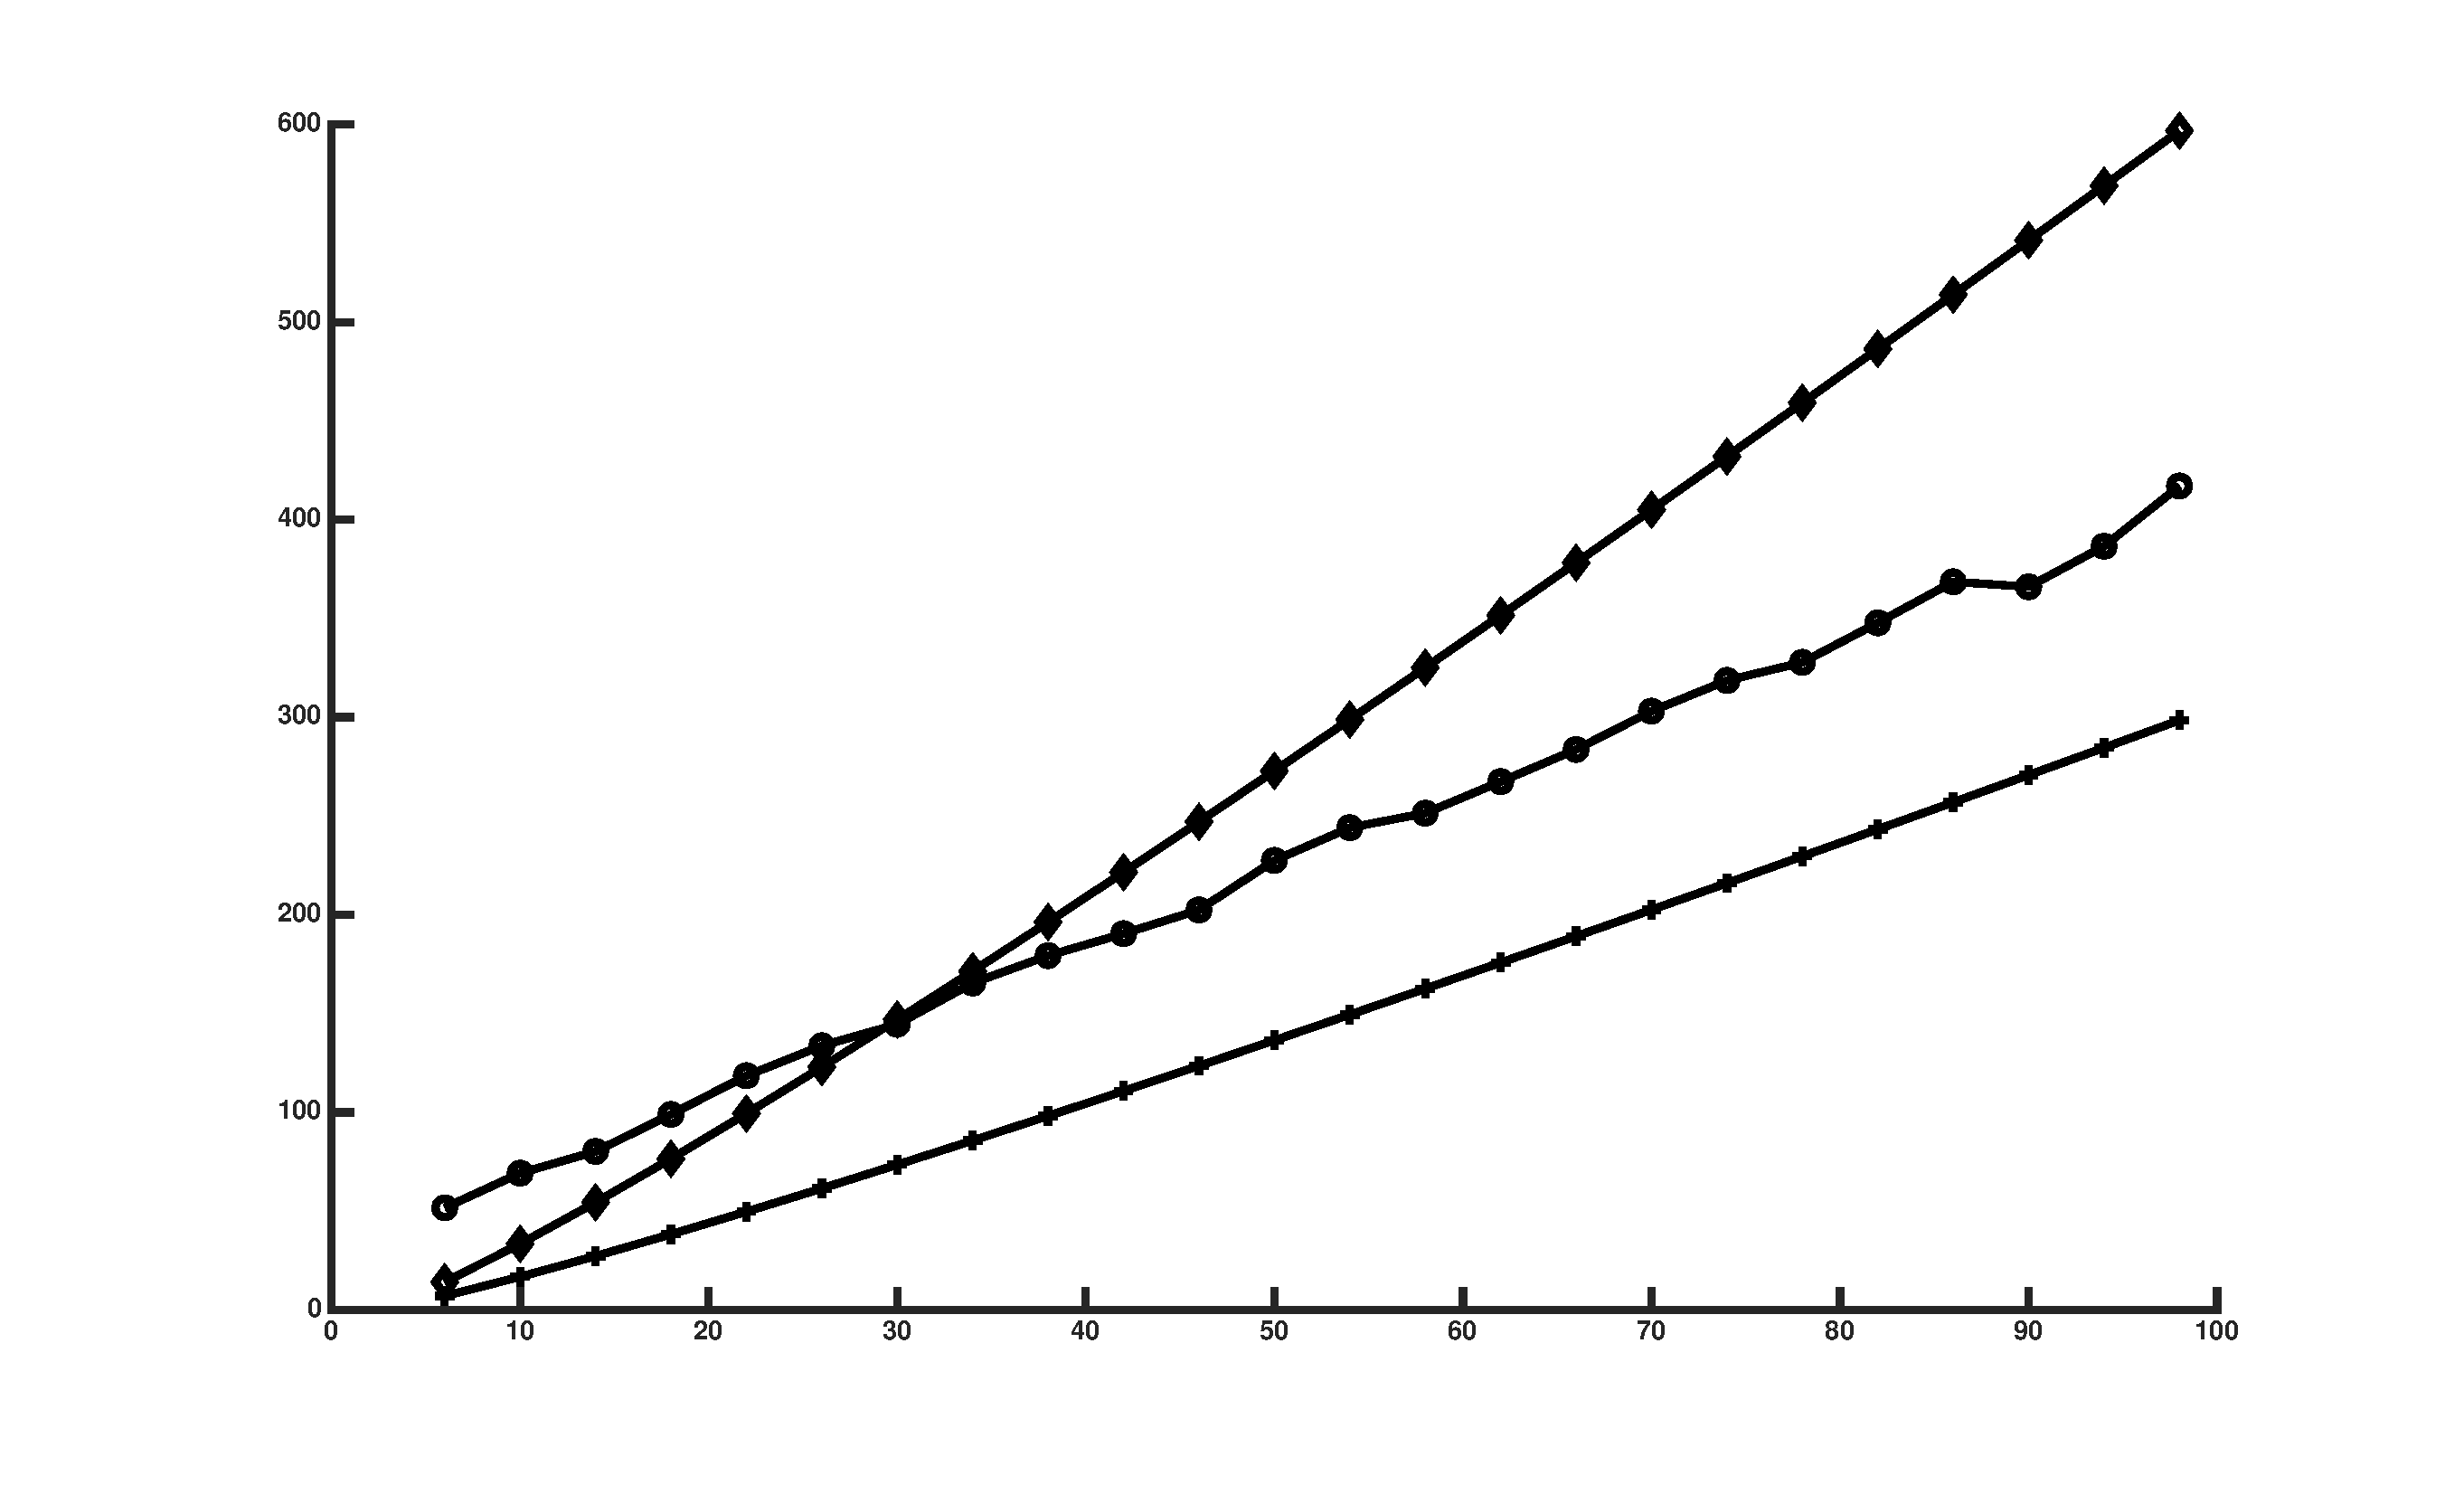
\includegraphics[trim = 0mm 10mm 0mm 10mm, clip, width=0.60\textwidth]{convTimes}
  \caption{Example~\ref{e:grow with n}, number of players vs. average convergence times. Here, there are two equal-sized populations of agents, $N_1$ and $N_2,$ and three resources $r_1,$ $r_2,$ and $r_3.$ 
Agents in population $N_1$ may choose from resources $r_1$ and $r_2,$ and agents in population $N_2$ may choose from resources $r_2$ and $r_3.$ Welfare functions are given in \eqref{e:welfares for another example}. \label{f:convTimes}}
\end{figure}

%\todo[inline]{Fix Figure~\ref{f:convTimes}, it is crooked.}

\end{example}


\begin{example}\label{s:large action sets}
In this example we investigate convergence times for modified log-linear learning when agents have larger action sets.   We consider the situation where $n$ agents are divided into two populations, $N_1$ and $N_2$. Agents in $N_1$ may choose from resources in $A_1 =\{r_1,r_2,\ldots,r_k\}$, and agents in population $N_2$ may choose from resources in $A_2 = \{r_k,r_{k+1}, \ldots, r_{2k-1}\}.$ That is, each agent may choose from $k$ different resources, and the two populations share resource $r_k$. Suppose resource welfare functions are
\begin{equation}\label{e:large action welfares}W_{r_j}(x) = 
\begin{cases}
x\mathop{/}4n  & \text{if } j\neq k\\
x^2\mathop{/}n^2 &\text{if } j=k,
\end{cases}
\end{equation}
and suppose agents' utilities are given by their marginal contribution to the total welfare, as in \eqref{e:MC util}. We allow $k$ to vary between 5 and 15, and $n$ to vary between 4 and 50. 

The welfare maximizing configuration is for all agents to choose resource $r_k$; however, when all agents in populations $N_1$ and $N_2$ choose resources $r_j$ and $r_{\ell}$ respectively, with $j,\ell\neq k,$ this represents an inefficient Nash equilibrium. Along any path from this type of inefficient Nash equilibrium to the optimal configuration, when $n\geq 4,$ at least $\lceil (n+4)/8\rceil$ agents must make a utility-decreasing decision to move to resource $r_k$. Moreover, the additional resources are all alternative suboptimal choices each agent could make when revising its action; these alternate choices further slow convergence times. Figure~\ref{f:LargeActionSets} shows the average time it takes to reach a configuration whose welfare is 90\% of the maximum, starting from an inefficient Nash equilibrium where all agents in $N_1$ choose resource $r_1$ and all agents in $N_2$ choose resource $r_{2k-1}.$ Parameter $\beta$ is selected so that the expected welfare is at least 90\% of the maximum in the limit as $t\to \infty.$ For each value of $k$, convergence times remain approximately linear in the number of agents, supporting Theorem~\ref{t:main theorem 1}.\footnote{In this example, convergence times appear super-linear in the size of populations' action sets. Note that the bound in \eqref{e:time requirement} is exponential in the the sum of the sizes of each population's action set.  Fast convergence with respect to parameter $s$ warrants future investigation; in particular, convergence rates for our log-linear learning variant may be significantly faster than suggested in \eqref{e:time requirement} under certain mild restrictions on resource welfare functions (e.g., submodularity) or for alternate log-linear learning variants (e.g., binary log-linear learning \cite{Arslan2007, Marden2007a}).}

\begin{figure}[ht]
  \centering
    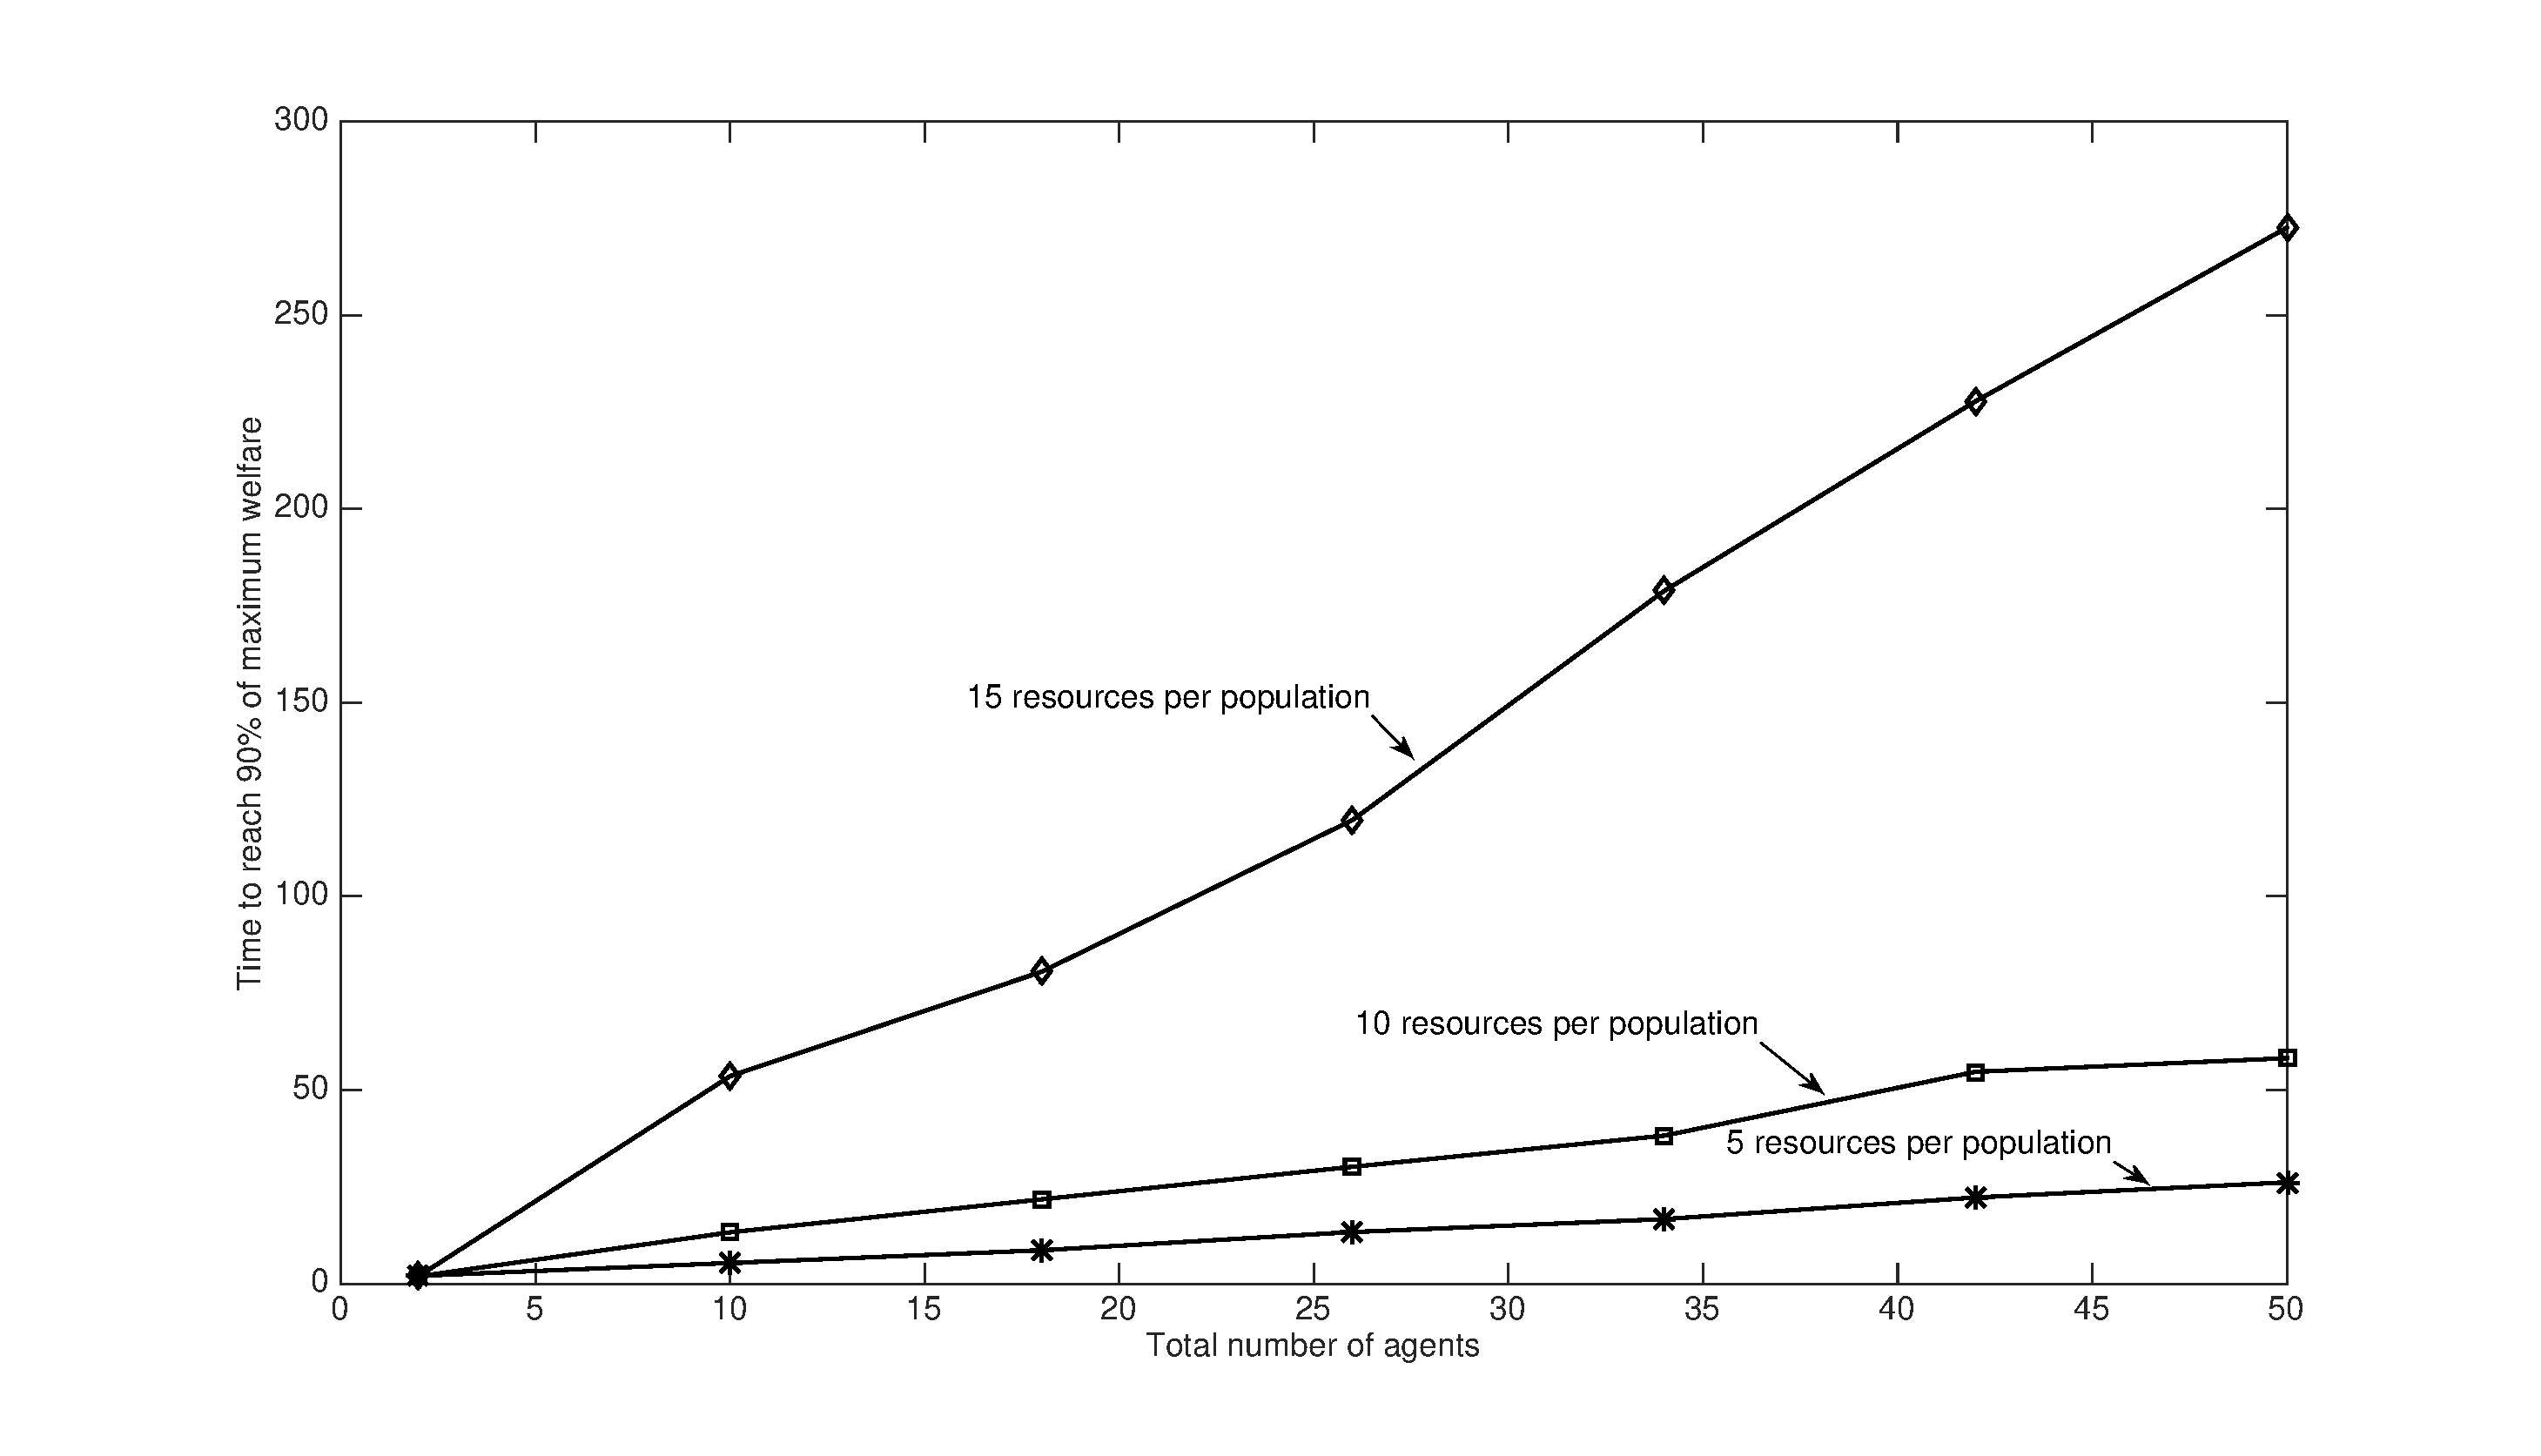
\includegraphics[trim = 40mm 10mm 40mm 20mm, clip, width=0.6\textwidth]{LargeActionSets}
  \caption{ ~\ref{s:large action sets}, number of agents vs. average time to reach 90\% of the maximum welfare. Agents are separated into two populations, $N_1$ and $N_2.$ Agents in $N_1$ choose from resources $r_1, r_2,\ldots,r_k$, and agents in $N_2$ choose from resources $r_k, r_{k+1}\ldots,r_{2k-1},$ where $k$ varies from 5 to 15. Resource welfare functions are given by \eqref{e:large action welfares}, agent utility functions are given by \eqref{e:MC util}, and average convergence times are taken over 200 simulations. \label{f:LargeActionSets}}
\end{figure}

\end{example}





In Example~\ref{e:SensorTarget} we compare convergence times for standard and modified log-linear learning in a sensor-target assignment problem.


\begin{example}[Sensor-Target Assignment]\label{e:SensorTarget}
In this example, we assign a collection of mobile sensors to four regions. Each region contains a single target, and the sensor assignment should maximize the probability of detecting the targets, weighted by their values. The targets in regions $R = \{r_1,r_2,r_3,r_4\}$ have values
\begin{equation}
v_1 = 1,\quad v_2 = 2,\quad v_3 = 3,\quad v_4 = 4\label{e:area vals}
\end{equation}
respectively. Three  types of sensors will be used to detect the targets: strong, moderate, and weak. Detection probabilities of these three sensor types are:
\begin{equation}p_s = 0.9,\quad p_m = 0.5,\quad p_w = 0.05.\label{e:detection probs}
\end{equation}
The numbers of strong and weak sensors are $n_s = 1$ and $n_m = 5.$  We vary the number of weak sensors, $n_w$.

The expected welfare for area $r_i$ is the detection probability of the collection of sensors located at $r_i$ weighted by the value of target $i$:
\begin{equation*}
W_{r_i}(k_s,k_m,k_w) = v_i\left( 1 - (1 - p_s)^{k_s}(1 - p_m)^{k_m}(1 - p_w)^{k_w}\right),
\end{equation*}
where $k_s,$ $k_m$ and $k_w$ represent the number of strong, moderate, and weak sensors located at region $r_i.$
The total expected welfare for configuration $a$ is
\begin{equation*}
W(a) = \sum_{r\in R} W_r(|a|_r^s,|a|_r^m,|a|_r^w),
\end{equation*}
where $|a|_r^s,|a|_r^m,$ and $|a|_r^w$ are the numbers of strong, moderate, and weak sensors choosing region $r$ in $a$.

We assign agents' utilities according to their marginal contributions to the total welfare, $W$, as in \eqref{e:MC util}. 
Our goal is to reach 98\% of the maximum welfare. We set the initial state to be a worst-case Nash equilibrium.\footnote{The initial configuration is chosen by assigning weak agents to the highest value targets and then assigning strong agents to lower value targets. In particular, agents are assigned in order of weakest to strongest according to their largest possible marginal contribution. This constitutes an inefficient Nash equilibrium. As a similar example, consider a situation with two sensors with detection probabilities $p_1 = 0.5$ and $p_2 = 1$, and two targets with values $v_1 = 2$ and $v_2 = 1.$ The assignment (sensor 1$\to$ target 1, sensor 2$\to$ target 2) is an inefficient Nash equilibrium, whereas the opposite assignment is optimal.  The large state space makes it infeasible to directly compute a stationary distribution, and hence also infeasible to compute values of $\beta$ that will yield precisely the desired expected welfare. Thus, we use simulations to estimate the $\beta$ which yields an expected welfare of 98\% of the maximum.}
 
To approximate convergence times, we simulate each algorithm with the chosen $\beta$ value\footnote{To approximate the value of $\beta$ which yields the desired steady-state welfare of 98\% of maximum, we simulated the standard and modified versions of log-linear learning for $1\times 10^6$ iterations for a range of $\beta$ values. We then selected the $\beta$ which yields an average welfare closest to the desired welfare during the final $5000$ iterations. Note that we could instead set $\beta$ according to \eqref{e:beta lb} for the modified log-linear learning algorithm; however, in order to compare convergence times of modified and standard log-linear learning, we chose $\beta$ to achieve approximately the same expected welfare for both algorithms.} and compute a running average of the total welfare over 1000 simulations. In Figure~\ref{f:SensorTarget} we show the average number of iterations necessary to reach 98\% of the maximum welfare.
 
For small values of $n_w$, standard log-linear learning converges more quickly than our modification, but modified log-linear learning converges faster than the standard version as $n_w$ increases. The difference in convergence times is significant ($\approx 1000$ iterations) for intermediate values of $n_w.$ As the total number of weak sensors increases, (1) the probabilities of transitions along the paths to the efficient Nash equilibrium begin to increase for both algorithms, and (2) more sensor configurations are close to the maximum welfare. Hence, convergence times for both algorithms decrease as $n_w$ increases. 


This sensor-target assignment problem does not display worst-case convergence times with respect to the number of agents for either algorithm. However, it demonstrates a situation where our modification can have an advantage over standard log-linear learning. In log-linear learning, the probability that the strong sensor will update next decreases significantly as the number of agents grows. In modified log-linear learning this probability remains fixed. This property is desirable for this particular sensor-target assignment problem, since the single strong sensor contributes significantly to the total system welfare. 


\begin{figure}[ht]
  \centering
    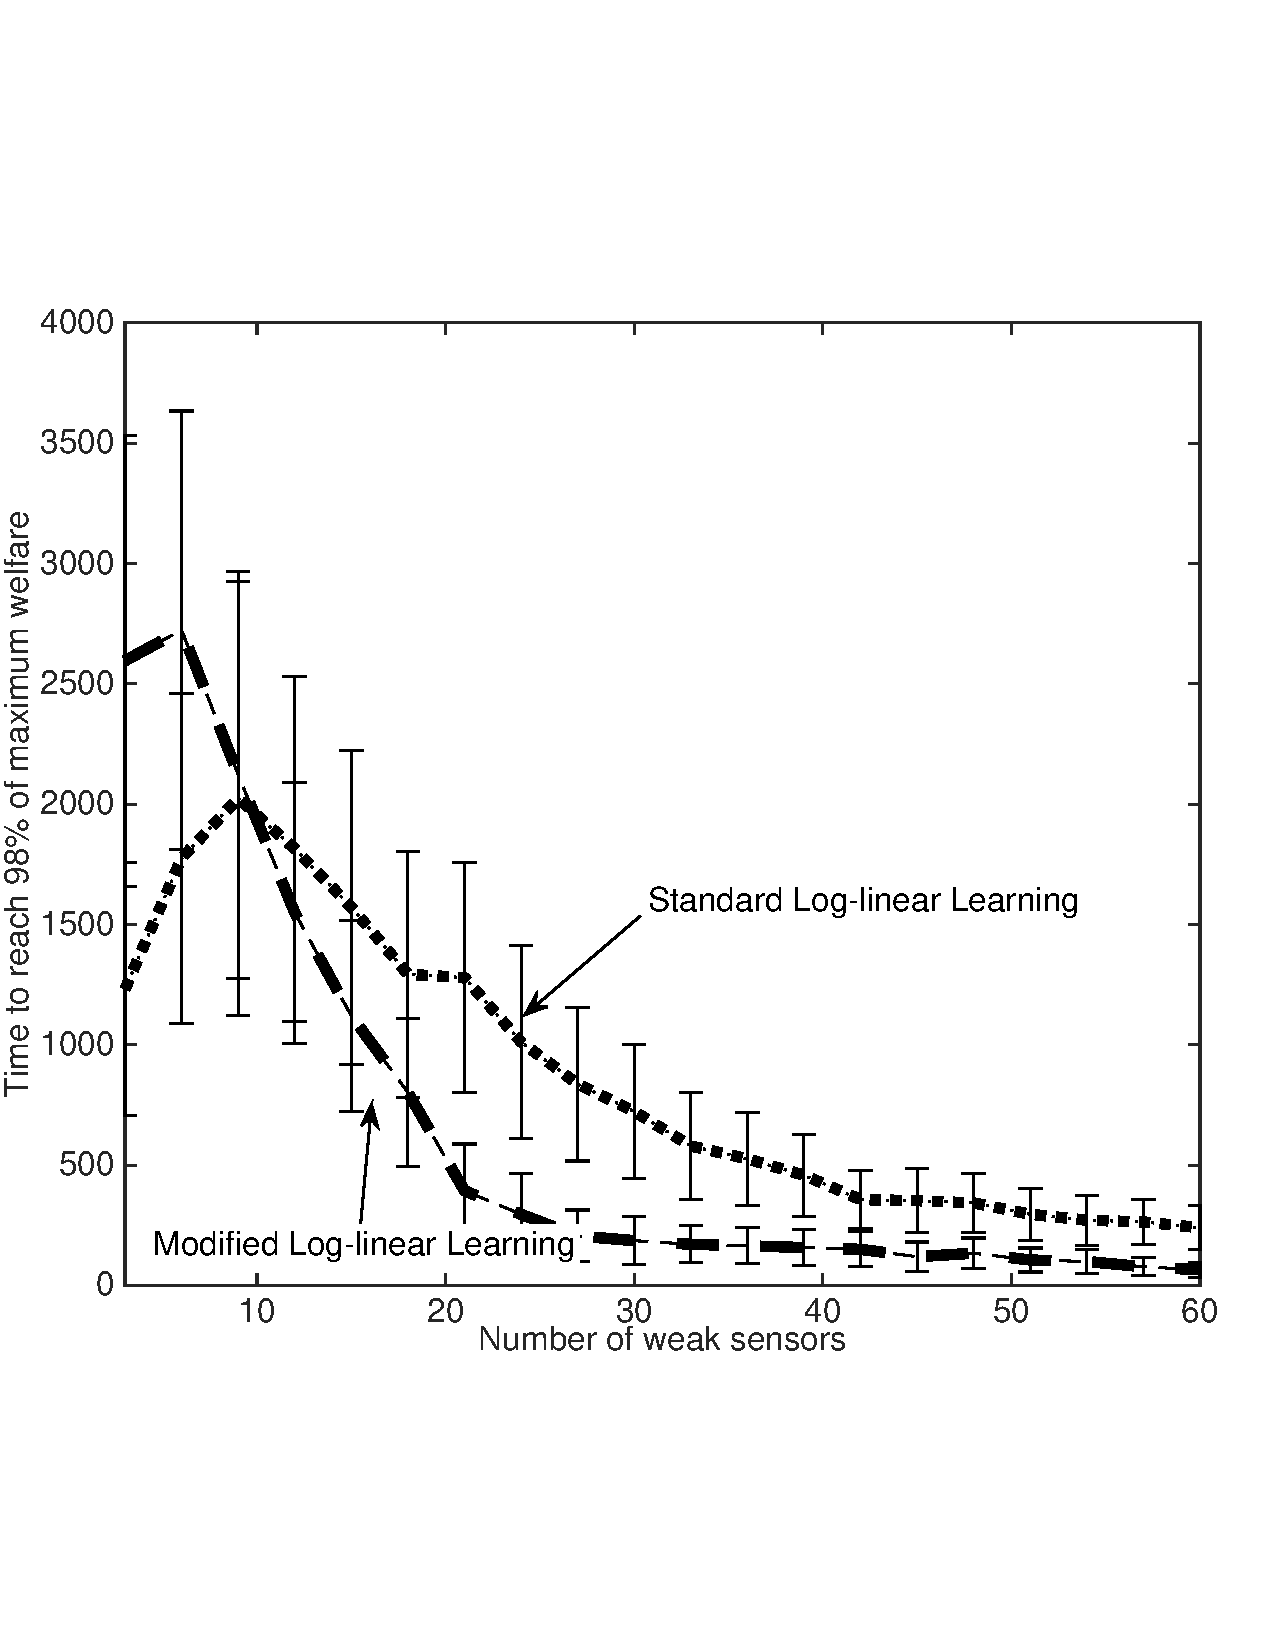
\includegraphics[trim = 0mm 40mm 0mm 40mm, clip, width=0.45\textwidth]{SensorTargetErrBars.pdf}
  \caption{ Example~\ref{e:SensorTarget}, number of weak sensors vs. average convergence times. Here, there are three types of sensors which may choose from four resources. Sensor detection probabilities and resource values are given in \eqref{e:detection probs} and \eqref{e:area vals}. We fix the number of strong and moderate sensors and vary the number of weak sensors. This figure shows the average time it takes for the average welfare to reach 98\% of maximum. The average is taken over 1000 iterations, and convergence times correspond to a global update rate of 1 per second. Error bars show standard deviations of the convergence times.\label{f:SensorTarget}}
\end{figure}

\FloatBarrier

\end{example}


%\section{Conclusion}

In summary, we have extended the results of \cite{Shah2010} to define dynamics for a class of semi-anonymous potential games whose player utility functions may be written as functions of aggregate behavior within each population.  For games with a fixed number of actions and a fixed number of populations, the time it takes to come arbitrarily close to a potential function maximizer is linear in the number of players. This convergence time remains linear in the initial number of players even when players are permitted to enter and exit the game, provided they do so at a sufficiently slow rate.

